\documentclass{beamer}

\usepackage[utf8]{inputenc}
\usepackage[T1]{fontenc}
\usepackage[ngerman]{babel}
\usepackage{amssymb}
\usepackage{amsmath}
\usepackage{amsthm}
\usepackage{graphicx}
\usepackage{caption}

% \usepackage{xcolor}
% \usepackage[Algorithmus]{algorithm}% http://ctan.org/pkg/algorithms
% \usepackage{algpseudocode}% http://ctan.org/pkg/algorithmicx
\usepackage{graphicx}
% \usepackage{wrapfig} % für grafiken mit textumfluss
\usepackage[font=footnotesize]{caption}
\captionsetup{format=plain}
\usepackage{ulem}
\usepackage{hyperref}
% \usepackage[colorlinks, linkcolor = black, citecolor = black, filecolor = black, urlcolor = blue]{hyperref} 


\title{Mathematische Spieltheorie}
\subtitle{Konkurrenz vs. Kooperation}
\author{Betreuer: Florian Thaler}
\date{Mai 2022}


% getting rid of navigation symbols in the lower right corner
\setbeamertemplate{navigation symbols}{}

\AtBeginSection[]
{
	\begin{frame}
		\frametitle{\normalsize Übersicht}
		\setbeamerfont{block title}{size=\normalsize}
		\normalsize
		\tableofcontents[currentsection]
	\end{frame}
}


\begin{document}


	\begin{frame}[plain]
		\titlepage
	\end{frame}

	\begin{frame}
		\frametitle{Gliederung des Vortrags}
		\tableofcontents
		% fußnote ohne nummerierung
% 		\let\thefootnote\relax\footnote{Durch * gekennzeichnete Abschnitte werden an der Tafel präsentiert.}
	\end{frame}

	\section{Einleitung}
		
		\begin{frame}
 			\frametitle{Motivierendes Beispiel}
            Florian und sein Lieblingsnachbar A
            \vspace{0.25cm}
 			\begin{columns}
				\begin{column}{0.25\textwidth}
					\begin{figure}[t]
						
\includegraphics[scale = 0.35]{images/fightingNeighbours}	
					\end{figure}
				\end{column}
				\begin{column}{0.5\textwidth}
                    \vspace{0.5cm}
					\begin{itemize}
                        \item Dünne Wände zwischen den Wohnungen
                        \item A ärgert sich über Florians (offenbar) zu laute Waschmaschine
                        \item Florian hingegen ärgert es wenn A laut Radio hört
					\end{itemize}
				\end{column}
			\end{columns}
		\end{frame}

        \begin{frame}
            \frametitle{Motivierendes Beispiel}
            Wie können die beiden Spieler in dieser Situation agieren?
            \begin{columns}
                \begin{column}{0.55\textwidth}
                    \begin{itemize}
                        \item Florian hat die Möglichkeit weiterhin seine Wäsche zuhause zu waschen oder sie in die Wäscherei
                            zu bringen.
                        \item Sein Nachbar kann sowohl laut aber eben auch leise dem Programm seines Lieblingssenders folgen. 
                    \end{itemize}        
                \end{column}
                \begin{column}{0.35\textwidth}
                    \begin{figure}
                        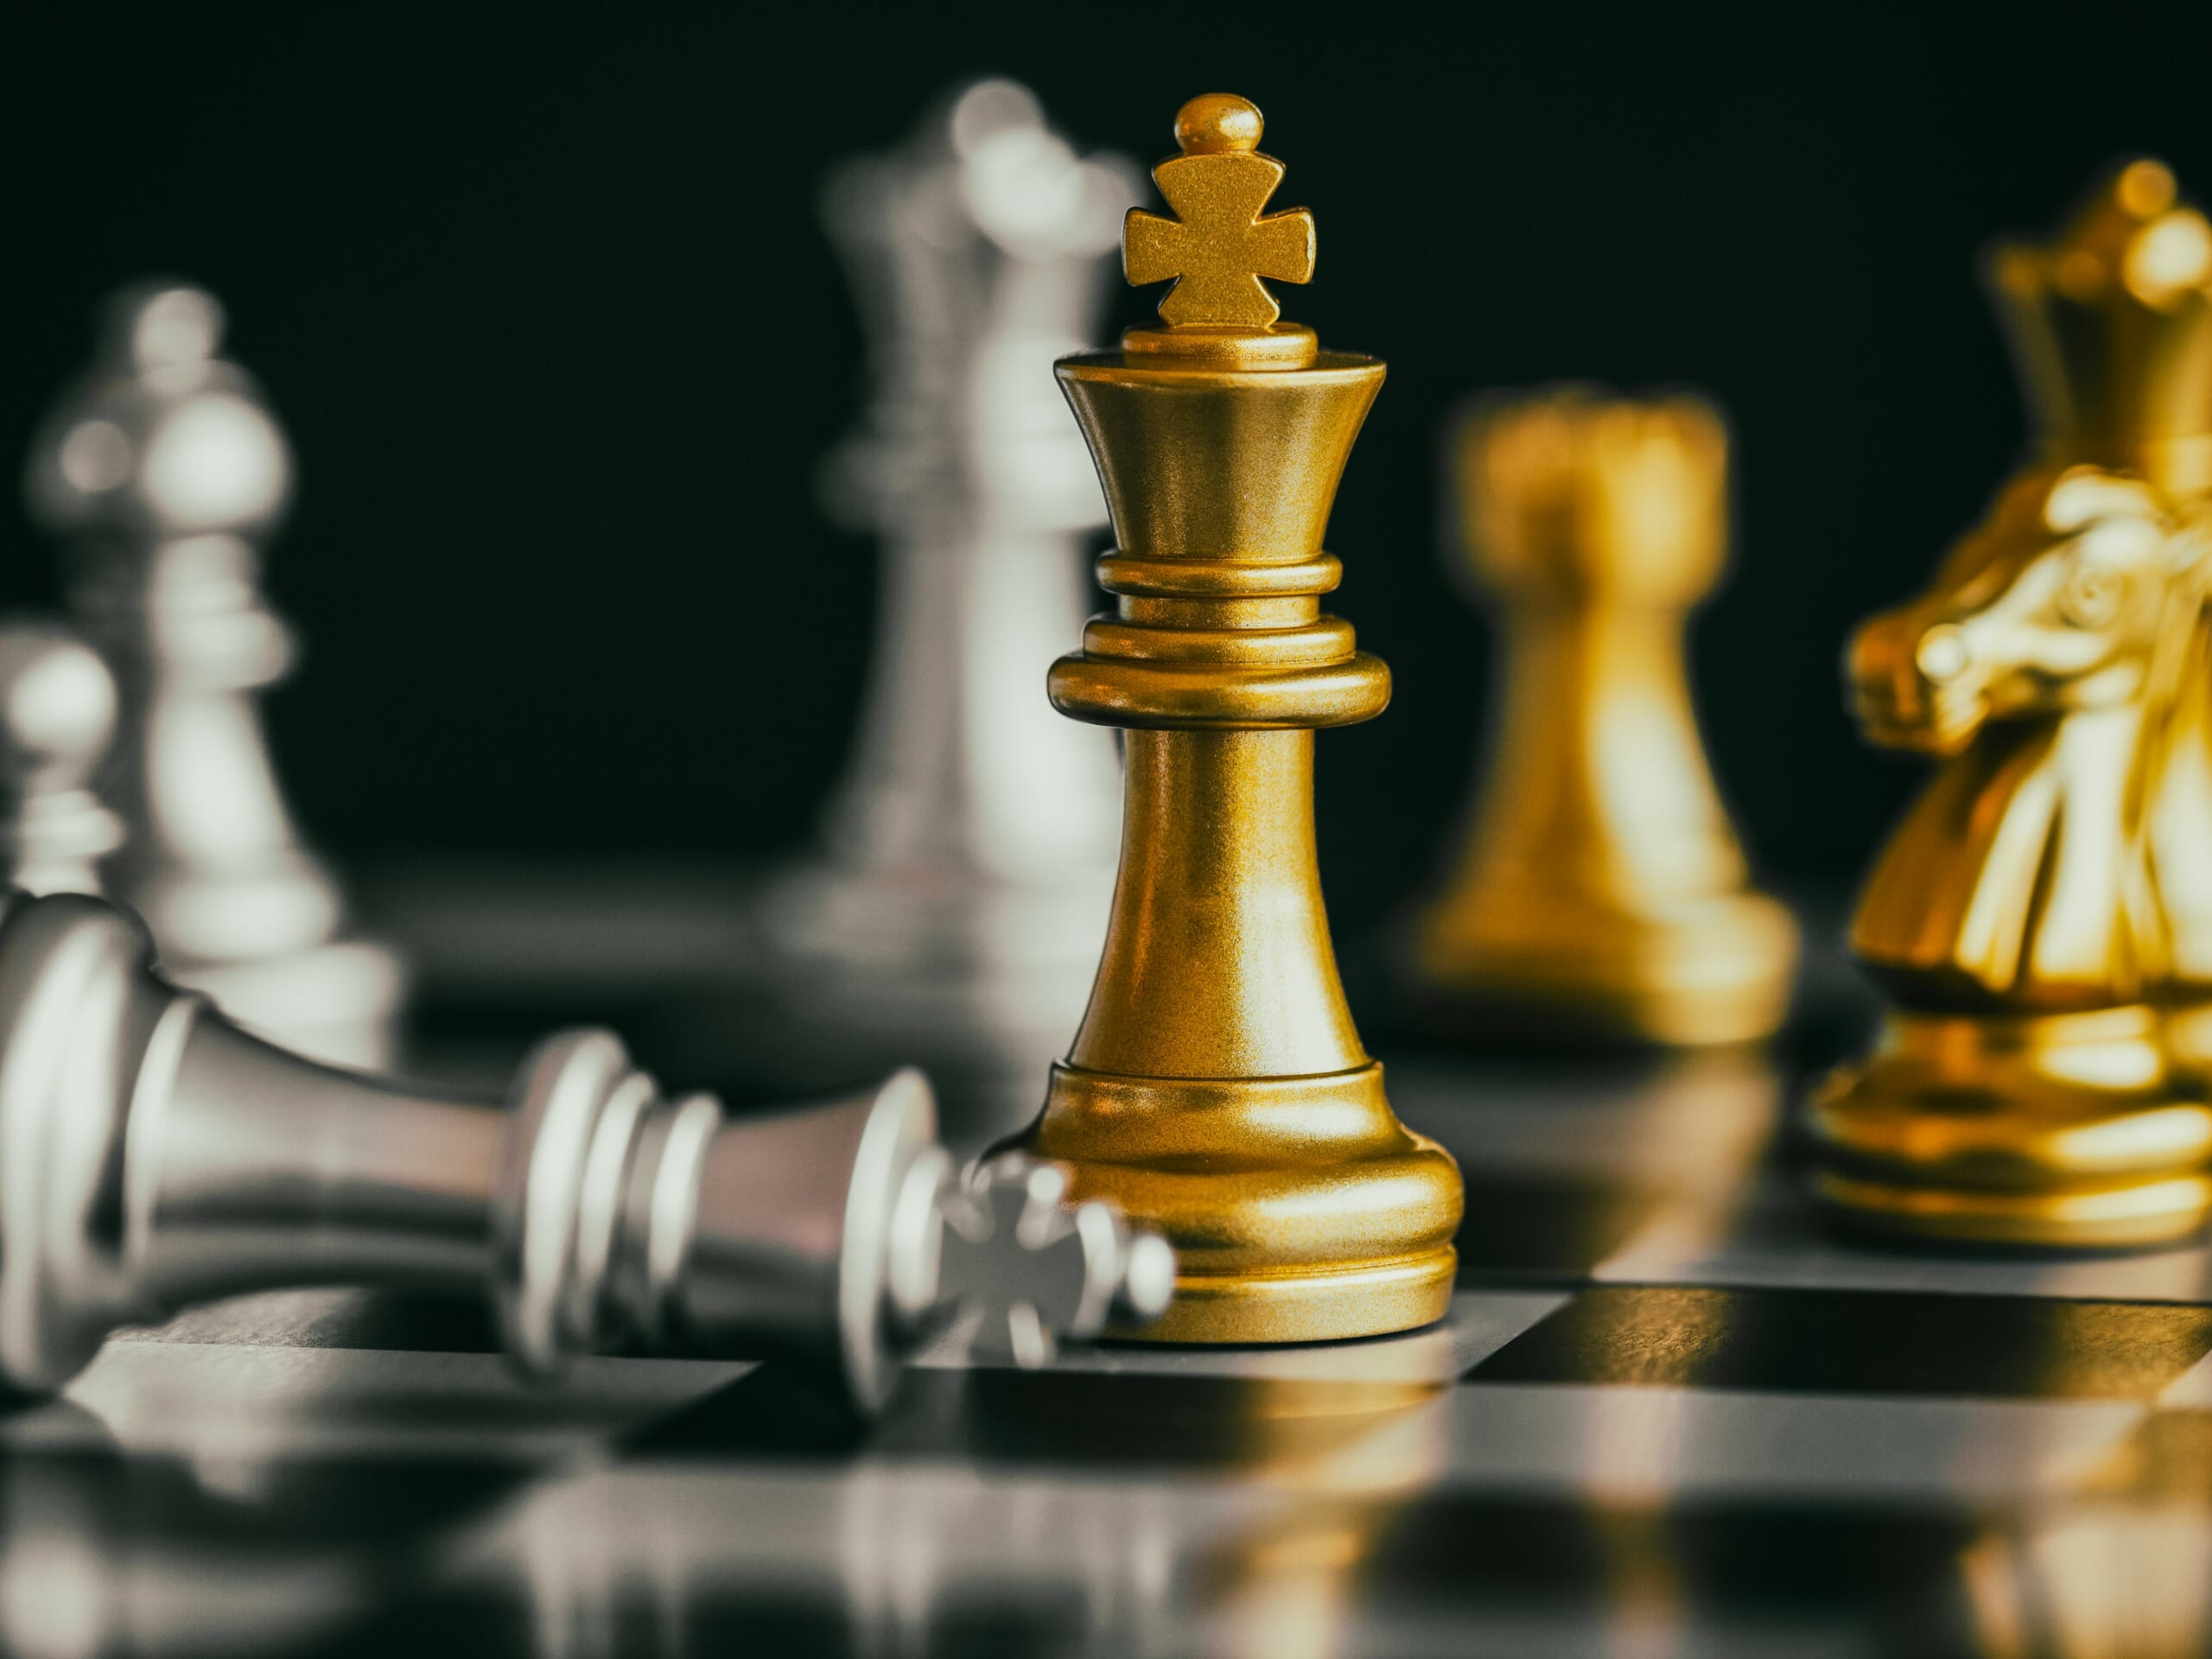
\includegraphics[scale = 0.045]{images/strategy_chess.jpg}
                    \end{figure}
                \end{column}
            \end{columns}
            \vspace{0.5cm}
            Welche Stragien sind die für Florian und seinen Nachbarn am gewinnbringendsten? Lohnt Kooperation?
        \end{frame}

        \begin{frame}
            \frametitle{Motivierendes Beispiel}
            Welche Stragien sind die für Florian und seinen Nachbarn am gewinnbringendsten? 
            \begin{columns}
                \begin{column}{0.25\textwidth}
                    \begin{figure}
                        
\includegraphics[scale = 0.3]{images/fightOrFlight.jpg}
                    \end{figure}
                \end{column}
                \begin{column}{0.55\textwidth}
                    \begin{itemize}
                        \item Konkurrenz oder Kooperation?
                        \item Gibt es alternive Strategien?
                    \end{itemize}
                \end{column}
            \end{columns}
        \end{frame}

    \section{Mathematische Spieltheorie}

		\begin{frame}
			\frametitle{Mathematische Spieltheorie}
            
			\begin{columns}
				\begin{column}{0.58\textwidth}
					\begin{itemize}
                        \item Modell einer \textbf{strategischen
                            Entscheidungssituationen} 
                            \begin{itemize}
                                \item \textbf{Rationale Akteure}
                                \item \textbf{Strategiemengen}
                                \item \textbf{Auszahlungsfunktion} oder Payoff-Funktion
                            \end{itemize}
                        \item Lösungskonzepte
                            \begin{itemize}
                                \item Nash Gleichgewichte
                                \item Minimax Stragien
                            \end{itemize}
					\end{itemize}
				\end{column}
				\begin{column}{0.48\textwidth}
					\begin{figure}
						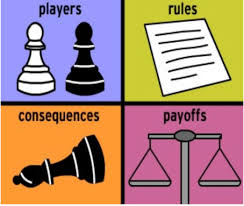
\includegraphics[scale = 0.45]{images/gameTheory.jpeg}
				% 		\caption{Regelkreis}
					\end{figure}
				\end{column}
			\end{columns}
		\end{frame}
		
	\section{Ziele des Projekts}
	
		\begin{frame}
			\frametitle{Ziele des Projekts}
			\begin{columns}
				\begin{column}{0.48\textwidth}
					\begin{figure}
						
\includegraphics[scale = 0.53]{images/projektziele.jpg}	
					\end{figure}
				\end{column}
				\begin{column}{0.5\textwidth}
					\begin{itemize}
						\item Modellierung von Entscheidungssituationen anhand geeigneter mathematischer Modelle
						\item Betrachtung verschiedener Ansätze zur Analyse von mathematischen Spielen
						\item Diskussion ausgewählter Probleme und Beispiel theoretisch als auch numerisch
						\item Last but not least:
                            \pause
                            \vspace{0.25cm}
                            \begin{center}
                                \large
                                \textbf{VIEL FREUDE AN DER MODELLIERUNG}
                            \end{center}
					\end{itemize}
				\end{column}
			\end{columns}
		\end{frame}

\end{document}
